\chapter{Related Work}
\label{ch:background}

% \todo[inline]{Gun: Again, it feels like you need better grouping of the sections as in the current structure, many of them overlap with each other, and it's a bit hard to see the logical flow of supporting why your thesis is important and how it fills in the research gap/limitation of the current state-of-the-art}

% \todo[inline]{Mark: This is important but probably should be in this section since it's not about virtual avatars. Maybe you need to have a section about information management, and discuss how these techniques could be used to manage avatar representations in Social AR.}

This work extends earlier work in wearable AR, AR annotation, social proximity, virtual avatars, research collaboration, telepresence, and sharing social experiences. This section examines previous related work on these areas of research and industry advancement, highlighting the gap in research and how this thesis attempts to explore new areas of research in AR social sharing. 

\section{Wearable AR} 

AR devices can be categorised into wearable (e.g., head-mounted displays, helmets or contact lenses), hand-held (e.g., phone, tablet) or projected displays where AR is projected onto a larger area regardless of where the user is looking~\cite{Peddie2017}. 

\textcite{Feiner1997a} presented the first mobile wearable AR system in 1997 called "The Touring Machine" combining a head-mounted display (HMD), hand-held tablet, and a backpack carrying a computer, GPS and radio for wireless access. This work was followed up by \textcite{Hollerer1999a} and explored different user interfaces on a wearable see-through display. The interface allowed users to sketch pathways and annotate their world for collaborative AR systems. 

Wearable AR has added an extra dimension to AR, allowing people to collaborate hands-free. \textcite{Feiner1999} talked about what impact wearable computing (and being mobile in general) has from the social perspective. These implications include personal privacy concerns, connectivity, collaboration, and how it looks and feels. 

Wearable AR has been explored for social interactions. For instance, \textcite{Cheok2002a} developed a city-wide wearable mixed reality social game, however, the system was bulky to wear, and they did not report on a user study. 

\textcite{Amores2015} used gestures to communicate social interactions via wearable devices. \textcite{Lee2019} used live 360 cameras to communicate between worker and helper. \textcite{Shu2018} developed a system of facial recognition to facilitate social interactions. 

With wearable AR devices becoming affordable, available and ubiquitous, there is a need to understand design considerations for this new platform. Previous research has looked into using AR headsets for collaborative use, for example in enhancing face-to-face \cite{Billinghurst2002} or remote collaboration \cite{Gupta2016}. The research presented here explores the use of AR headsets for social interaction and shared experiences. Social interactions can be extrapolated from current social network interactions where \enquote{friends} share content and interact with another's content (i.e., placing likes and comments).

\textcite{Dey2018} reviewed ten years of research in AR usability studies and highlighted the importance of user studies in AR research, especially the social and environmental impact of user studies that take place in outdoor locations. Remote collaboration is one of the main categories of AR user studies, but surprisingly, the number of research publications is relatively low until around 2014. They also reported that the increased availability of hand-held and wearable devices enabled for more research in this area. 

AR in remote collaboration was studied and found that AR was enhancing task completion \cite{Kim2014, Tversky2015, Gupta2016, Kim2015}.
\textcite{hauber2008understanding} studied remote video collaboration focusing on spatial interactions. In four experiments, the author measured the social presence, awareness, physical presence, co-presence, ease of use and efficiency between different conditions including immersive and virtual environments as well as standard video conferencing. Those experiments found higher social presence in video collaborative virtual environments compared to standard video conferencing and found that standard video or face to face collaboration was better than adding avatars in virtual collaboration.

% \todo[inline]{Again, what did you learn from these works? Your related-work section reads more like a laundry list of previous papers, rather than a set of papers that you read and learned something from, thereby informing your own choices and work. You've (rightfully) chosen to structure your related work section around larger themes, since this makes sense in terms of your own work. Now you need to help the reader understand what the papers you cite have done to help you.}

% There is a need to understand design considerations for this new platform. Previous research has looked into using wearable AR headsets for collaborative use, for example, in enhancing face to face \cite{Billinghurst2002} or remote collaboration \cite{gupta2016you}. The research presented here explores the use of AR headsets for social interaction and shared experiences. 

\section{AR Annotation}

There are several examples of AR annotation demonstrations on mobile devices \cite{Wither2009a, Gauglitz2014, Larabi2018, Grasset2012}. For example, mobile AR browsers (e.g., Wikitude\footnote{https://www.wikitude.com/} or Junaio\footnote{https://en.wikipedia.org/wiki/Junaio}) can overlay AR tags on the real world using GPS and other motion sensors. While they were successful in demonstrating the concept of visualising AR annotations, the registration of virtual objects in the real world could be inaccurate, and they could only be used in outdoor, large-scale environments. Mobile AR browsers usually create AR tags in advance, but  AR research projects have investigated in situ and interactive creation of AR tags. For example, \textcite{Kim2011} presented an interactive method where the user stands in a fixed position to calibrate the room model with the gyroscope data. The user can then touch and annotate locations with a rectangle where virtual content, like text, images and 3D models, can be overlaid. 

A variety of AR annotation methods with wearable interfaces have also been presented. SixthSense \cite{Mistry2009a} used a wearable gestural interface for AR annotation. It consisted of a camera and a small projector mounted on a hat or in a pendant. The camera tracked user hand gestures, and the projector visually augmented virtual content onto the physical objects with which the user is interacting. However, the system required planar surfaces in front of the user for accurate projection because of the lack of a depth sensor. OmniTouch \cite{Hollerer1999a} was a wearable projection system equipped with depth-sensing technology that enabled interactive multi-touch applications on different surfaces. Both the depth camera and projector are mounted onto a form-fitting metal frame, which is worn on the shoulders, and secured with a chest strap. This system extended the typical scenarios supported by SixthSense to on-body surfaces or objects held in hand for image projection. However, the system was still bulky and inconvenient to use because it needed to be connected to a desktop computer.

\section{Remote Collaboration}

\begin{figure}
    \centering
    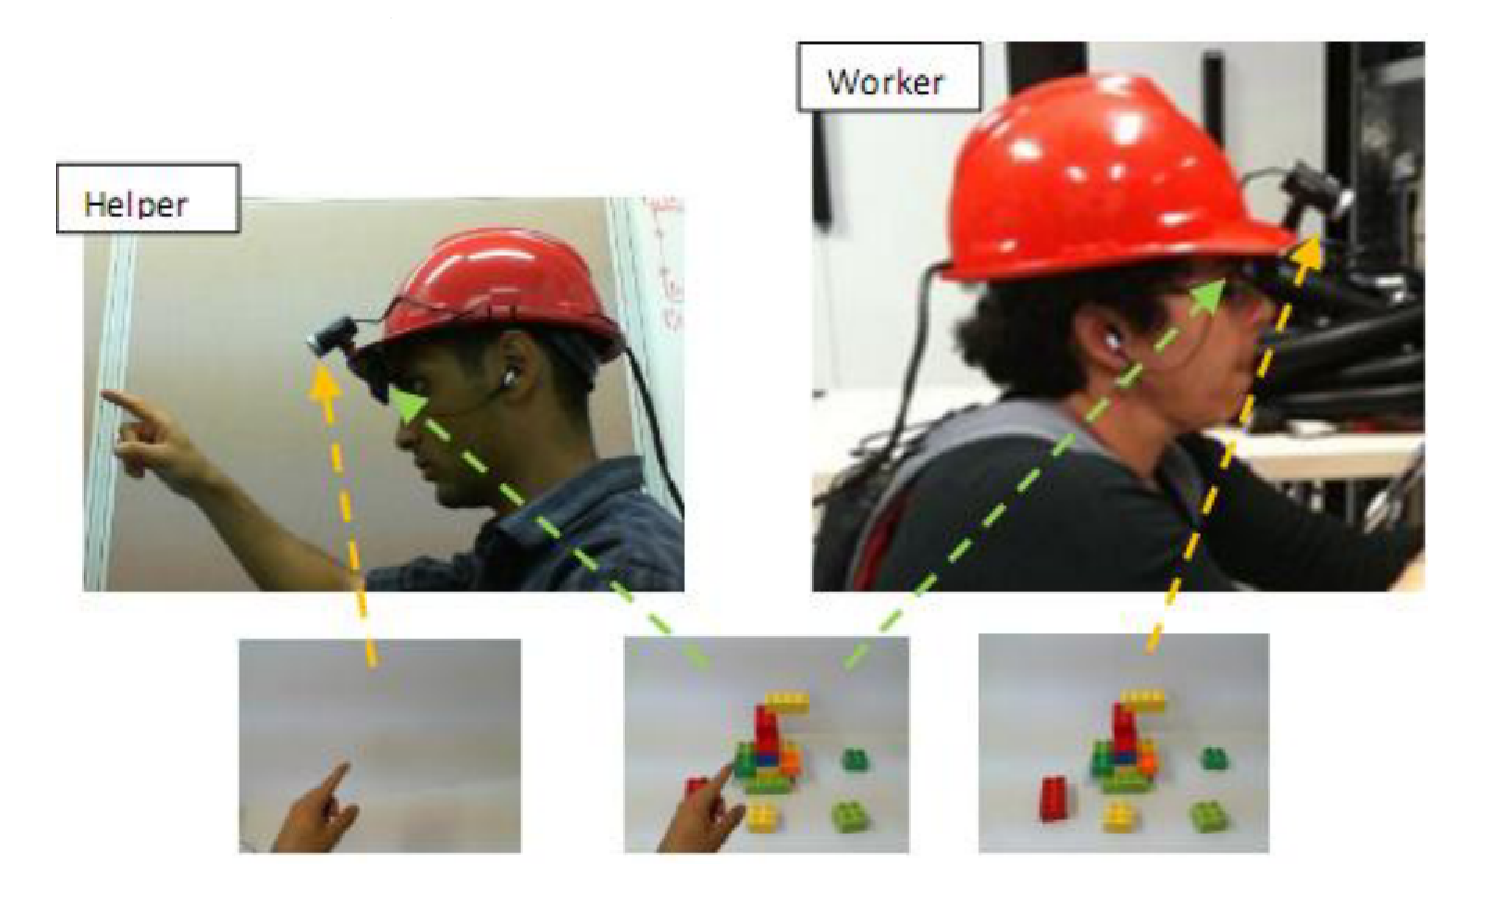
\includegraphics[width=\linewidth]{images/20-background/huang2013.eps}
    \caption{HandsInAir: A Wearable System for Remote Collaboration. The worker video share their work environment to the helper. The helper share their hand gestures to the worker during the remote collaboration session \cite{Huang2013}}
    \label{fig:HandsInAir}
\end{figure}

Camera-equipped mobile devices provide a quick way of capturing and sharing experiences and spaces. Wearable computers that combine HMDs and cameras provide new opportunities for collaboration. For example, the Google Glass\footnote{http://www.google.com/glass/} wearable system has a camera, microphone, and head-worn display.

There has been a significant amount of earlier research on remote collaboration using head-mounted cameras and displays. For example, allowing a remote user to place virtual annotations on the live camera view from a head-worn camera and showing the result in the wearers HMD, has been shown to enhance remote collaboration \cite{Fussell2003}. Other systems allow a remote user to place their hands in the local user's view~\cite{Huang2013} (Figure \ref{fig:HandsInAir}). 

In many wearable and mobile AR applications, remote collaboration is the primary purpose of sharing a view of the user's world. For example, remote expert collaboration systems have been developed where a local worker with an AR display can share a live video view of their workspace with a remote expert (Figure \ref{fig:Billinghurst2002}) \cite{Billinghurst2002}. The remote expert can provide visual feedback with AR graphical cues.  However, most of these systems have just been developed for collaboration between small numbers of users, and not for more extensive social networks. 

\begin{figure}
    \centering
    \includegraphics[width=\linewidth]{images/20-background/billinghurst2002.eps}
    \caption{Live virtual video avatars for remote collaborative AR interfaces. \cite{Billinghurst2002}}
    \label{fig:Billinghurst2002}
\end{figure}

\textcite{Muller2017} introduced adding shared virtual markers to help remote collaboration to be more effective and to understand the context of the collaboration. They found that the communication behaviour was improved and ambiguity was reduced in addition to enhancing the user experience. 

\section{Telepresence}      % why telepresence is relevant here

When remote people connect using telepresence techniques, they may also want to share different amounts of information about their surroundings with each other. For example, users who are close friends in a social network may be happy to share a 3D virtual view of their surroundings and have the remote user appear as an AR avatar in their real space, while those that are strangers may only want to have an audio connection and not show anything of their surroundings to preserve their privacy \cite{Oetzel2011}. 

\textcite{Fuchs2014} (Figure \ref{fig:Fuchs2014}) studied telepresence via a scanned 3D environment to enable social connections with people and simulated face-to-face interactions. The remote person was scanned and reconstructed live in the local environment. They forecasted that 3D telepresence was going to be more popular when technology becomes more capable.

\begin{figure}
    \centering
    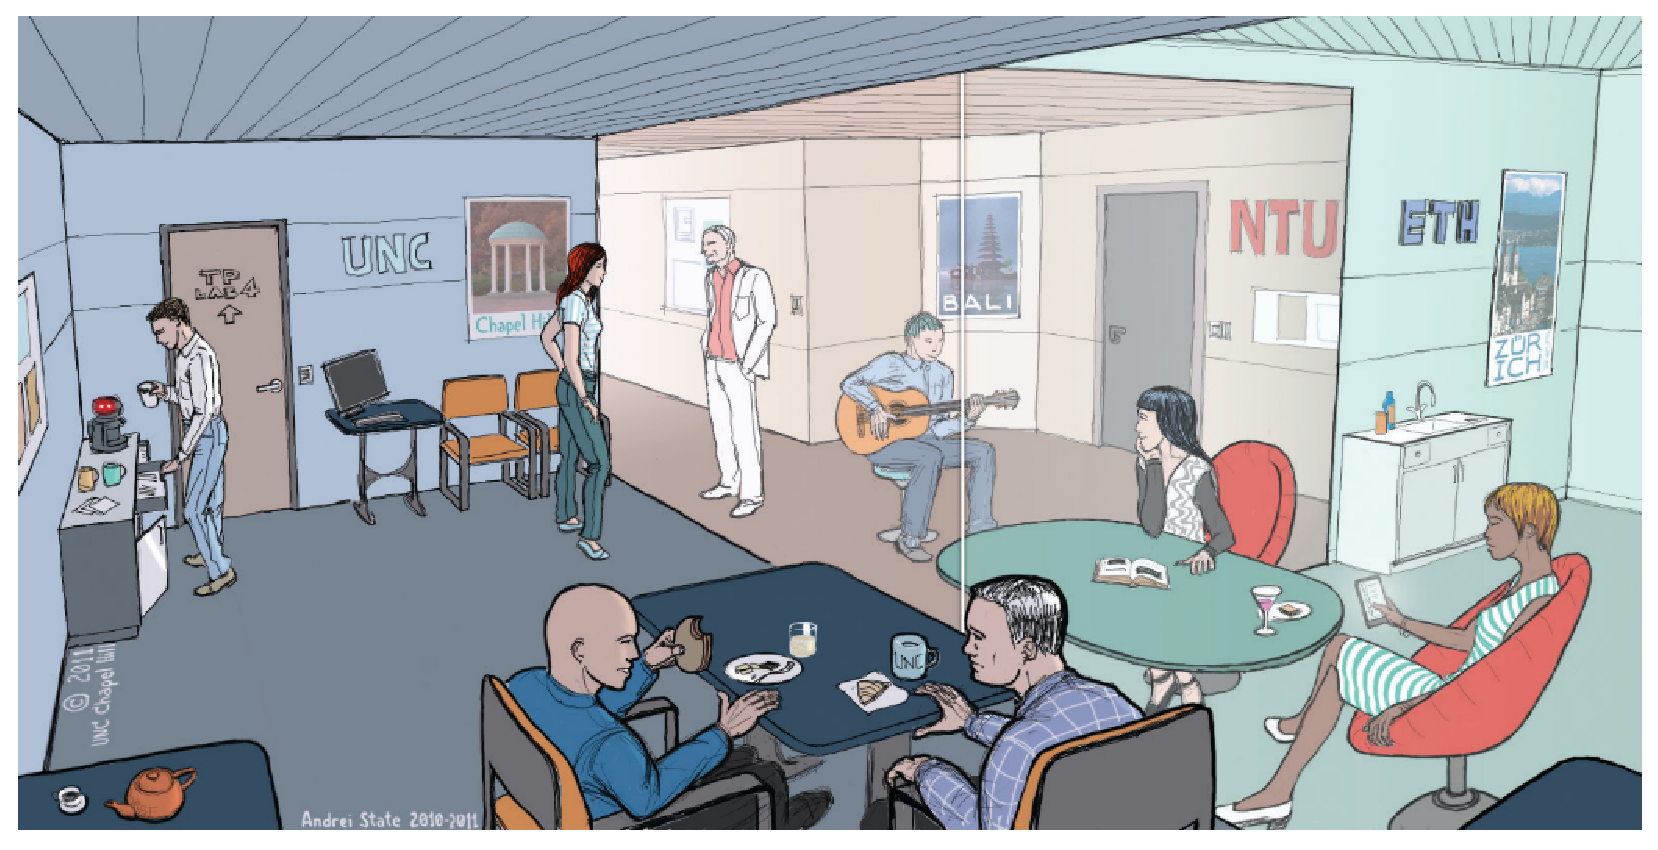
\includegraphics[width=0.6\linewidth]{images/20-background/fuchs2014_2.eps}
    \includegraphics[width=0.35\linewidth]{images/20-background/fuchs2014.eps}
    \caption{(left) The vision of sharing spaces and teleprsence by sharing social experiences beetween pysical space and virtual space. \\
    (right) Real-time 3D reconstruction of 2 humans sharing a social experience. The top images shows the depth image without colour, bottom images shows colour addition to depth data. The right images show the 3D images after correction for occlusion and filling missing data of 3D scans. \cite{Fuchs2014}}
    \label{fig:Fuchs2014}
\end{figure}


\section{Social Networks}

Previous work looked into social interactions in AR \cite{Schmalstieg_144, Xu2008, Xu2011, Faas2010}. \textcite{Schmalstieg_144} built a hand-held game to test social interactions between players and found that mobility gives an advantage of making the game socially enjoyable and engaging. \textcite{Xu2011} reported on social interaction observation on a tabletop board game. The game is played through hand-held AR devices. They discovered five categories of social interactions: 1) chores, 2) reflecting on gameplay, 3) deciding strategy of play, 4) game itself and 5) out of game subjects. They found that chore-based social interactions are richer interactions and help the users to be more emotionally connected, which increases the engagement throughout the game. AR was used to enhance social presence and create more engaging experiences in video-based communications \cite{Almeida2012}. \textcite{Almeida2012} built a prototype to segment the hand and overlay it on the video stream to create shared space experiences.

Advancements in mobile phone hardware and increased network connectivity have made live video streaming apps popular among smartphone users \cite{Liu2008}. Live video streaming apps have been used for sharing social experiences in various contexts. For instance, a person attending a conference or a concert could use their mobile phone to stream the event to their friends and family who could not be there. Similarly, live video streaming apps have also been used for social journalism \cite{Lenzner2014}, turning laypersons into live reporters. Consequently, these apps are now available from different sources with applications such as Periscope\footnote{https://www.periscope.tv/} and Facebook Live\footnote{https://live.fb.com/} among the most popular. These apps allow the users who are sharing to receive comments on the video they are sharing and to receive simple graphical feedback. 

Characteristic features of live-streaming apps include using the phones' camera which can be either pointed outward (recording what the user sees) or inward (where the user appears in the video) to allow users to send a live video stream of what they are doing to hundreds or even thousands of viewers. The purpose of sharing the video is social, so the experience is improved if the viewer can also provide feedback.

\begin{figure}
    \centering
    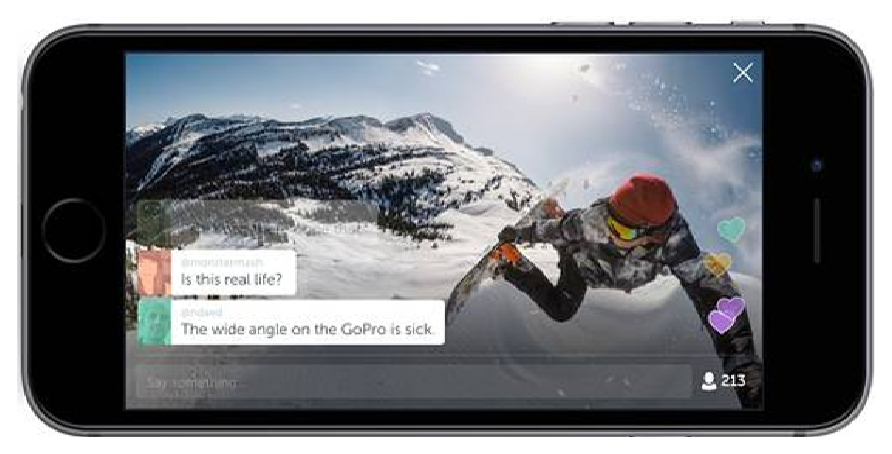
\includegraphics[width=0.4\linewidth]{images/20-background/periscope.eps}
    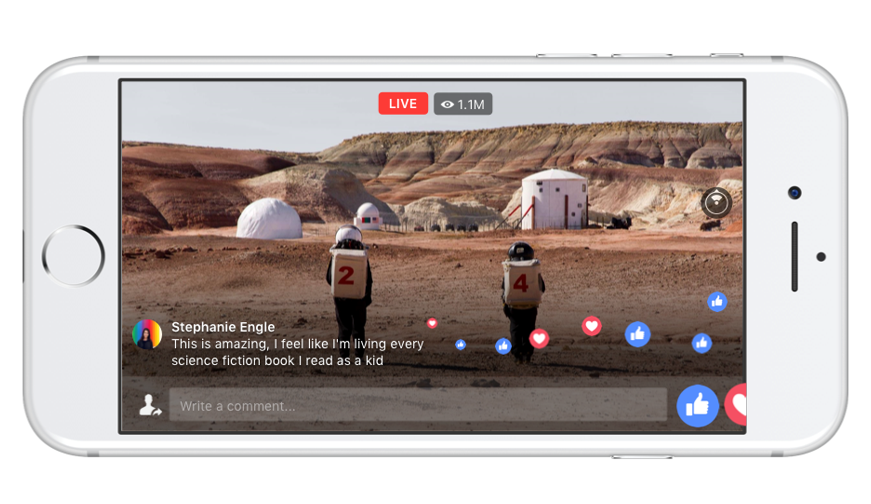
\includegraphics[width=0.4\linewidth]{images/20-background/facebook-live.eps}
    \caption{Examples of live-streaming apps: Periscope (left) and Facebook Live (right). Note the user interface of comments from viewers are displayed as a list on the UI.}
    \label{fig:live-streaming}
\end{figure}

In these applications, the feedback comments usually appear in a list below or beside the video being shared (Figure \ref{fig:live-streaming}), separate from the visual context of what the viewer is commenting on. This may cause problems when the person sending the video changes their viewpoint. For example, a viewer might send the comment "I like that view", but by the time the comment appears, the view might already have changed from the view being commented on.

Future social interactions with wearable AR can be extrapolated from current social network interactions where friends share content and interact with others' content on mobile platforms such as Facebook and Instagram. For example, Facebook Live allows a person with a mobile phone to live stream to remote collaborators. Similarly, wearable AR systems have already been developed that enable people to share a view of their surroundings. For example, the Shared Sphere work of \textcite{lee2017mixed} allows a user with a wearable AR display to live-stream a 360-degree video of their surroundings to a remote collaborator, although only between pairs of users. 

\section{Social Proximity}

For representing "people" in AR space, \textcite{Sousa2016} (Figure \ref{fig:Sousa2016}) studied the concept of \enquote{personal space} and \enquote{social bubbles} in terms of proxemic interactions between people in different places. They used floor projections and hand-held devices to communicate the presence of remote people. They also established a \enquote{gradual engagement model for remote proxemics} based on the distance from the user, which consisted of 1) personal, 2) engaged, 3) peripheral and 4) ambient.

\begin{figure}
    \centering
    \includegraphics[width=0.8\linewidth]{images/20-background/sousa16.eps}
    \caption{Gradual engagement model for remote proxemics representing four levels: 1) personal, 2) engaged, 3) peripheral and 4) ambient. \cite{Sousa2016}}
    \label{fig:Sousa2016}
\end{figure}

\textcite{Leshed2012} studied different representations of social relationships and identity in Second Life and found that people use metaphors such as onion layers to represent layers of their identity, gradually revealing as the interpersonal relationship developed between people. \textcite{Hans2009} explored the connection between social proximity and social temperature (e.g., warm feeling and cold shoulder) and found that there is a link between social proximity, language and perception. 

% \cite{Gergle2004}

Most previous work has focused on how visual representation and proximity could be used to organise an AR representation of a person's social network. However, this information could also be used to modify the contextual information being shared by a user out to their social network as well. 

\section{Virtual Avatars}

In the social AR/VR space, previous work implemented a variety of visual representations of self and others. For example, \textcite{Fanello2016} prototyped live sharing of a full scan of a person's body with remote users using 3D cameras and the HoloLens\footnote{https://www.microsoft.com/en-nz/hololens}. 

Scanning a person body in 3D has become more accessible on a consumer scale. For instance, Echo Look by Amazon\footnote{\url{https://en.wikipedia.org/wiki/Amazon\_Echo\#Echo\_Look}} is a 3D depth camera that people can use pose in front of, and use AR to overlay different outfits on themselves to see how they would look before purchasing the outfit. The user can share photos of themselves wearing a few outfits with their friends to get feedback on which outfit would look better. 

Similarly, some companies (such as High Fidelity\footnote{https://highfidelity.com/}, Sansar\footnote{https://www.sansar.com/}, Itsme3D\footnote{https://www.itsme3d.com/} and other VR shared worlds) are building social VR experiences in which users are represented as 3D virtual avatars. For instance, virtual avatars have been used to share social experiences such as in Facebook Spaces\footnote{https://www.facebook.com/spaces} (Figure \ref{fig:facebook-spaces}) where users can meet in VR, take selfies and teleport to a 360-degree video. Virtual avatars for self and others are represented as a floating face and upper body rendered in a VR background. 

360-degree videos have been studied as a medium for Mixed Reality enabled remote collaboration tasks \cite{Tang2017a, Lee2017, lee2017mixed, Lee2019}. Results show that by using 360-degree videos, the remote user can have an independent view of the local person and be able to achieve higher co-presence and be more effective in task completion. 

\begin{figure}
    \centering
    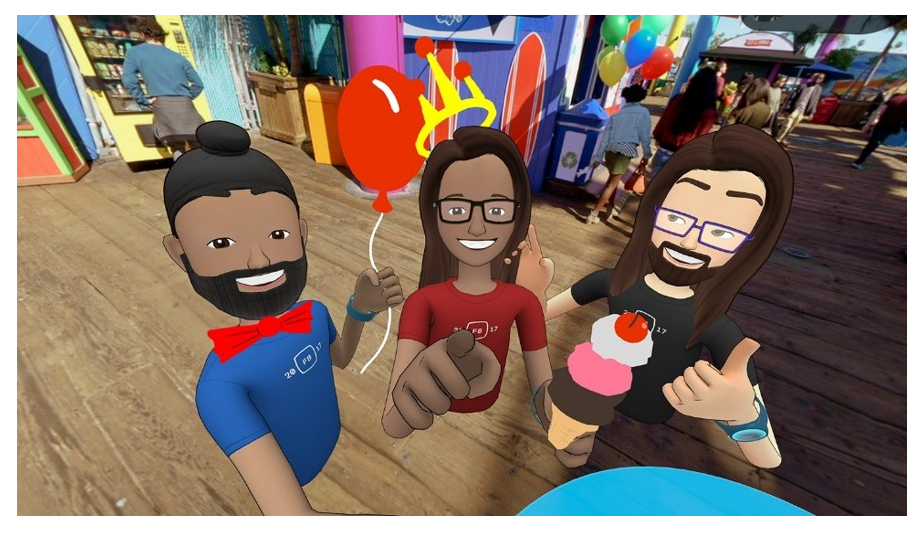
\includegraphics[width=0.8\linewidth]{images/20-background/facebook-spaces.eps}
    % 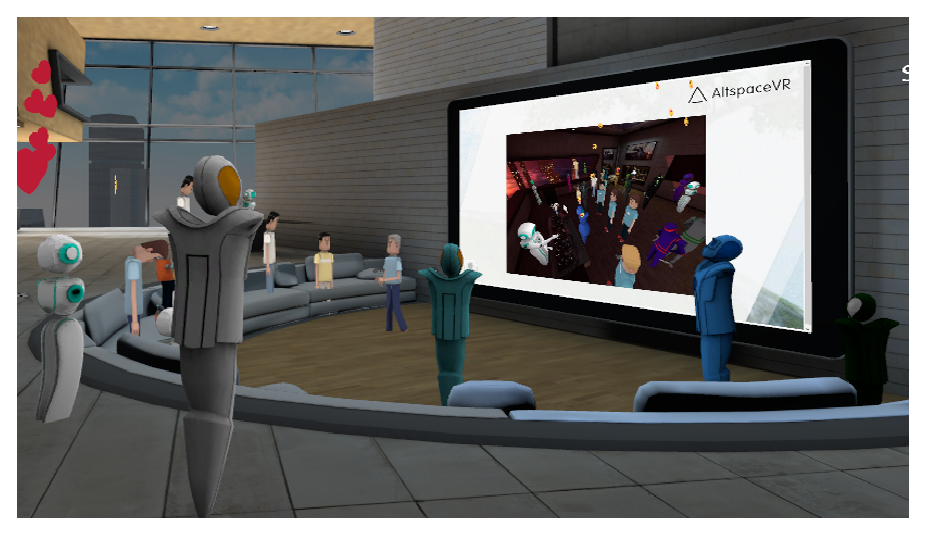
\includegraphics[width=0.4\linewidth]{images/20-background/altspace-vr.eps}
    \caption{Example of avatars in VR. Facebook Spaces}
    \label{fig:facebook-spaces}
\end{figure}

As for the social AR spaces, there have been limited examples of social applications. Avatar Chat was introduced by Magic Leap\footnote{https://www.magicleap.com/experiences/social} (Figure \ref{fig:ml-avatar-chat-2}) in late 2018. The app allows users to connect with their social contacts and view their avatar overlaid on top of their physical environment. Users can share emojis, connect to a group "avatar" chat and talk about images overlaid in their space. The avatars are cartoonish-looking representing the upper half of the body floating in the AR space. Natural hand gestures are detected using the depth cameras on the device, assisted by computer vision algorithms and translated to a pre-defined set of virtual hand gestures to the other participants in the chat session. 

Saptiate\footnote{http://spatiate.com/} is another social app launched in early 2019 on Magic Leap where users can connect in a chat session with primitive avatars, sketch in their AR world, and share the sketching in real-time with connected users. The users can see each other's avatars and hear their voices. 

\begin{figure}
    \centering
    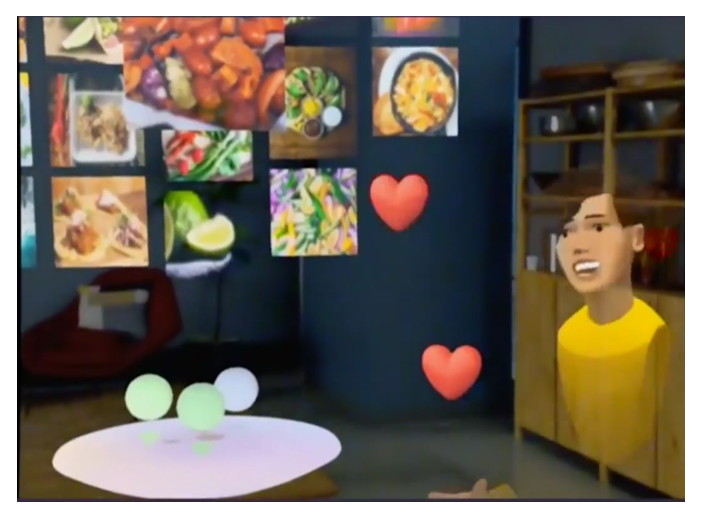
\includegraphics[width=0.8\linewidth]{images/20-background/avatar-chat-1.eps}
    % 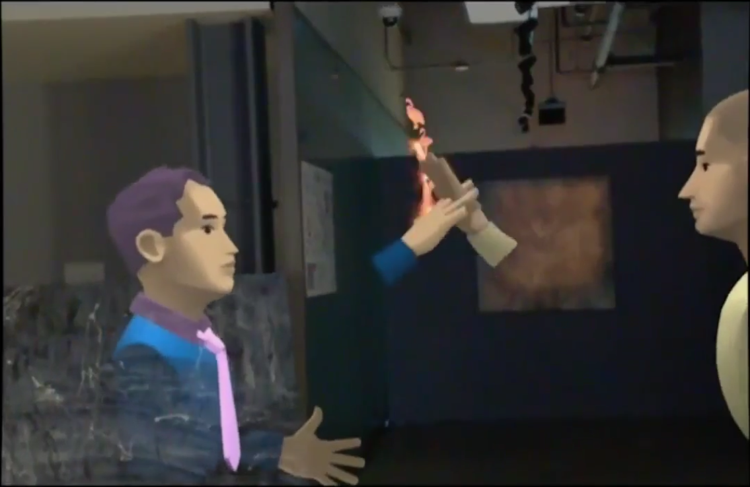
\includegraphics[width=0.4\linewidth]{images/20-background/avatar-chat-2.eps}
    \caption{Example of avatars in AR - Avatar Chat by Magic Leap}
    \label{fig:ml-avatar-chat-2}
\end{figure}

However, representing social contacts in VR/AR can be cumbersome. It can be more cluttered and overwhelming to represent the data content that social avatars are trying to share. Futuristic concept videos have imagined social data (e.g., "Hyper-Reality" \footnote{https://www.youtube.com/watch?v=YJg02ivYzSs} and "Merger" \footnote{https://www.youtube.com/watch?v=SqW2dEkiD-Y}) where social data can clutter the AR view of the user. It will also raise privacy and ethical concerns.

\textcite{Greenwald2017} studied social presence in room-scale VR. They used virtual avatars for communicating and collaboration in a social setting. They found that using embodied avatars in VR interactions is practical for collaboration tasks with the benefit of social presence. One of the tasks was drawing to communicate, which was challenging for participants. 

\textcite{Jo2016} studied the influence on co-presence of the background environment (AR vs VR) and the fidelity of the avatar representation of the remote user (photo-realistic vs pre-built). They found that more realistic avatars had a positive impact on the feeling of co-presence between remote collaborators. \textcite{Volante2016} also studied the impact of the visual appearance of avatars (realistic vs. stylised) on the inter-personal emotional response of participants. They also found that more visual realism has lower adverse effects on the PANAS scale, which measures the intensity of the emotion at a given time. Researchers have been investigating the social aspects of multi-user VR environments. \textcite{Ducheneaut2006} studied massive multiplayer online games in terms of social activities, and found that while users may prefer to be with other players, they do not necessarily like actively interacting with them. This led us to think that users may want to have the sense of the presence of social contacts around them, but not necessarily interact with them.

\textcite{Harris2009} studied the social behaviour of users of Second Life\footnote{secondlife.com} and found that users became less active over time and went to familiar places rather than being explorative and actively teleporting/flying. They found out that people prefer routine and to be surrounded by familiar faces/places over time, forming a social group.

% mark: [you should about how they handle crowds or if everyone is just represented the same] 
However, there has been very little research into social representation in AR. The AR space is challenging in terms of finding the best locations to fit avatars in the real world, so they do not interfere with physical objects or appear suspended in mid-air. However, a social AR application could also allow people to see their friends while doing other tasks; users do not have to use an immersive VR environment to see their social contacts.

Researchers have also explored different ways of managing a large number of information tags in AR interfaces. \textcite{Julier2002} showed how environmental cues, such as distance and user context, can be used to filter AR content into the most relevant information. \textcite{Hollerer2001} describe how can the view management techniques be used to ensure that virtual objects can be easily seen in collaborative AR interfaces. Similarly, \textcite{Grasset2012} show how an image-based approach can be used to ensure AR information tags do not overlap in hand-held AR. 

This previous research shows that visual fidelity can be used to distinguish between virtual avatars. Different visual representations and spatial cues can also be used to distinguish between information tags in an AR interface. However, there has been little or no research on how to manage social network representations in AR for large numbers of connections. The next section explores how visual and proximity cues could be used to organise contacts in a wearable social AR interface.

% \todo[inline]{[In this section, you should probably also mention how VR Virtual Avatar environments handle hundreds or more simultaneous users. For example, what tools does second life have for connecting people to hundreds of others? This is directly relevant to your thesis topic]}


%----------------------------------------------------------------------------------------
%    Summary
%----------------------------------------------------------------------------------------
\section{Summary}

This work aims to layout the space of the Social AR Continuum for social sharing experiences by looking at parameters and options that can be changed in terms of people, objects and the environment to create a shared AR experience. 

Building on previous work on proximity-based relationships \cite{Sousa2016}, this work focuses on the shared contents of social avatars in an asynchronous situation. Unlike previous work on social avatars, this thesis studies representing social contacts in a large-scale network. The aim of this work is to reduce the clutter that may be caused by displaying social avatars and their shared content. This thesis addresses the question of how we can use the social relationship between avatars and the viewer as a way to filter and enhance viewing the shared-content experiences. 

The scope of this thesis is to explore options of visual user experience design in social AR, including displaying contacts, displaying shared data, and displaying shared environments. This thesis does not necessarily cover all possible experiences but highlights the main points of interactions and reports on user studies measuring the sense of presence and privacy concerns that may occur from these experiences. 

The summary of the trends in the past work is that wearable AR has been the target of many previous developments and research directions. Aiming to enable true outdoor experiences and to be untethered to physical places would allow more exploration of the surrounding world. 
Most of the previous work in AR collaboration was focused on task-oriented situations where a remote expert is assisting a local worker to complete a particular task, which is useful in manufacturing and technical industries.
In the social aspects of AR, previous work showed few attempts of representing social networks in AR and VR. 
% Also, some applications looked into scanning and using human avatar representations for social connections with others.

The limitation of past work is that it was mainly focused on the remote collaboration of local worker/remote helper situations. However, it did not address sharing social experiences with friends and family. There is some new work in this area, but not enough to cover all dimensions in this field. The gap that this thesis is addressing is the user interaction design of future wearable AR interfaces so that AR can be easily used for sharing social experiences with family and friends. 

The research in this thesis is important because it explores different ways of presenting social networks on wearable AR and helps application designers and developers by providing insights into building similar applications that have a higher chance of being effective and acceptable to users. 

The contributions to the current state-of-the-art are: 1) building software prototypes of sharing social experiences on wearable AR platforms, 2) Running user studies on these prototypes and analysing the results, 3) providing the foundations of the design space of sharing social experiences on wearable AR. 

% \todo[inline]{Gun: You should have a paragraph summarising the trend in the past work and what is the limitation to support why your work is important. Or you may add a section at the end of this chapter that does an overall review of the whole chapter and describe how your thesis makes a contribution to the current state-of-the-art.}

% \todo[inline]{You should end the chapter with a summary of the research gap that you're going to be addressing.}

% \todo[inline]{[At the end of the related work section you should have a sub-section that provides a summary of the research, particularly highlighting the research gaps and shortcomings of this earlier work. You can then talk about which aspects you are going to explore further in your PhD thesis. Highlight what the novelty of your thesis is, and what will be the main contributions that your research will make, relative to the earlier related work] }

% \subsection{Sharing for Collaboration}
% \subsection{Sharing for Social}

